\documentclass[a4paper, 15pt]{article}
\usepackage[left=0.85in, right=0.85in, top=0.5in, bottom=0.95in]{geometry}
\usepackage[T1]{fontenc}
\usepackage[utf8]{inputenc}
\usepackage[italian]{babel}

% Formattazione del testo
\usepackage{setspace}         % Setting dello spazio\begin{spacing}{0.95}
\setstretch{1.2}
\setlength{\parindent}{0pt}
\raggedbottom
\usepackage[none]{hyphenat}    % no sillabazione 
\usepackage{multicol}          % testo su più colonne
\usepackage{changepage}	       % \begin{adjustwidth}{}{}

% Matematica
\usepackage{amsmath, amssymb, amsthm, mathtools}
\usepackage{cancel}            % semplificazioni \cancel{expression}
\newtheorem*{thm}{Teorema}
\newtheorem*{en}{Enunciato}
\newtheorem*{definizione}{Definizione}
\newtheorem*{cor}{Corollario}
\DeclareMathOperator{\rk}{rk}
\DeclareMathOperator{\im}{Im}

% Simboli e Disegni
\usepackage{color}             % \textcolor{'ColorCode'}{'testo'}
\usepackage{graphicx, wrapfig, float}
\usepackage{tikz, circuitikz}
\usetikzlibrary{patterns, arrows, decorations.markings, arrows.meta, decorations.text}
\tikzset{immagine/.style={above right, inner sep=0pt, outer sep=0pt},
	testo/.style={fill=white, align=center, fill opacity=0.6, text opacity=1, below, font=\sffamily\bfseries\footnotesize}}
\usepackage{pgfplots}
\pgfplotsset{compat=1.15}
\usepackage{mathrsfs}

% Altri pacchetti
\usepackage{enumitem}
\usepackage{mdwlist} 	       % suspend enumerate \suspend{} \resume{}
\usepackage{siunitx}
\sisetup{
	% output-decimal-marker = {,},  % preferisco i punti, sono più leggibili
	list-final-separator = { e },
	list-pair-separator = { e },
	range-phrase = { a }
}
\usepackage{hyperref}
\hypersetup{
	colorlinks=true,
	linkcolor=blue,    
	urlcolor=blue,
}
\urlstyle{same}

% Altre definizioni personali
\usepackage{pifont}
\newcommand{\cmark}{\ding{51}}
\newcommand{\xmark}{\ding{55}}
\DeclareUnicodeCharacter{20AC}{\EUR}
\newcommand{\compresslist}{\setlength{\itemsep}{1pt}\setlength{\parskip}{0pt}\setlength{\parsep}{0pt}}
\newcommand{\ra}[1]{\renewcommand{\arraystretch}{#1}} % stretcho le tabelle e gli array \ra{x}
\setlength{\jot}{10pt}


% Titolo e data
\title{9. Misure di temperatura}
\date{}

\begin{document}
	\maketitle
	\setcounterpageref{secnumdepth}{0}
	\setcounter{tocdepth}{5}    
	\begin{spacing}{0.95}
		\tableofcontents 
	\end{spacing}
	\newpage
	
\section{Scale termometriche}
\begin{adjustwidth}{2in}{}
	I sensori di temperatura sono stati sviluppati piuttosto "tardi" principalmente perché questa è una grandezza fisica intensiva, e quindi definibile sono attraverso gli effetti provocati dalle sue variazioni sul comportamento dei materiali e poi perché ovvero non è correlabile a grandezze fisiche sensibili. \newline 
	
	La temperatura descrive infatti lo stato termodinamico di sistemi che sono in equilibrio ed è funzione dell'energia cinetica media posseduta dalle molecole: questa non può essere direttamente misurata. \newline
	
	Come definire una scala termometrica? Magari individuando dei punti caratteristici di riferimento, come quelli del cambiamento di stato.
	
	Potrebbe essere utilizzata una barra di rame immersa in una miscela a temperatura nota e registrare le variazioni di volume del materiale in funzione della variazione di temperatura della miscela, ma questo porterebbe ad una definizione di scala termometrica dipendente dalla tipologia di materiale utilizzato. \newline 
	
	Nel corso della storia scienziati e filosofi hanno cercato di fornire una scala termometrica universalmente accettabile, la prima di queste è senza dubbio la \textbf{scala Fahrenheit} (1724), in cui per la sua realizzazione si utilizzò un bulbo di vetro graduato con all'interno del mercurio, questo caratterizzato da coefficiente di espansione costante e buona leggibilità. 
	
	Si vengono ad individuare così le seguenti temperature
	\begin{itemize}
		\item Solidificazione dell'acqua: 32 gradi
		\item Ebollizione dell'acqua: 212 gradi
		\item Uomo sano: 96 gradi
	\end{itemize}
	
	Un'altra scala termometrica universalmente accettata è la \textbf{scala Celsius} (1742), in questa si individuano invece
	\begin{itemize}
		\item Solidificazione dell'acqua: 0 gradi
		\item Ebollizione dell'acqua: 100 gradi
	\end{itemize}
	Dividendo l'intervallo in 100 parti uguali. \newline
	
	Queste scale termometriche si basano sull'utilizzo di un materiale, il mercurio e sono sostanzialmente differenti tra loro, per cui arriva la necessità di assolutizzare tale scala e renderla il più possibile indipendente dal materiale utilizzato per definirla. 
	
	Si passa così all'utilizzo di gas (1780) i quali, a bassa pressione e al di sotto delle loro temperature critiche, mostrano comportamenti pressoché identici e variazioni lineari del volume con la temperatura a pressione costante e viceversa.
\end{adjustwidth}
\newpage
\subsection{Scala termodinamica del gas perfetto}
\begin{adjustwidth}{2in}{}
	Questa scala termodinamica si basa sull'utilizzo di gas perfetti per cui
	\[P_T = P_0(1+\alpha_V)T \Rightarrow T = \dfrac{P_T-P_0}{\alpha_VP_0} = 100\cdot\dfrac{P_T-P_0}{P_{100}-P_0}\]
	In cui si è sostituito, dalla formula
	\[P_{100} = P_0(1+\alpha_V)100\]
	Dove 
	\begin{itemize}
		\item $P_T$ è la pressione del gas ideale alla generica temperatura $T$ espressa magari in \unit{\degreeCelsius}
		\item $P_0$ è la pressione del gas ideale a \SI{0}{\degreeCelsius}
		\item $P_{100}$ è la pressione del gas ideale a \SI{100}{\degreeCelsius}
		\item $\alpha_V$ è il coefficiente di temperatura di un gas ideale a volume  costante [\unit{\per\degreeCelsius}]
	\end{itemize}
		Tuttavia, anche in questo caso sorgono alcune criticità
	\begin{itemize}[label=\textcolor{red}{\xmark}]
		\item Incertezza associata al valore di $\alpha_V$
		\item Definizione vincolata al gas utilizzato: nella realtà si utilizza un gas reale
	\end{itemize}
	Esiste tuttavia un metodo per \textbf{correggere} il comportamento del gas reale: fargli compiere una trasformazione isocora, a volume costante.
	\begin{figure}[H]
		\centering
		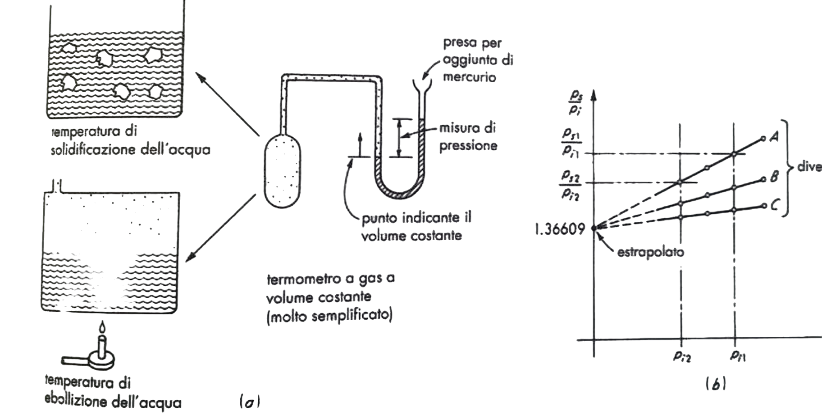
\includegraphics[width=0.4\linewidth]{immagini/screenshot001}
		\label{fig:screenshot001}
	\end{figure}
	$T_r$ e $P_r$ sono la temperatura e la pressione scelte come riferimento (punto triplo dell'acqua)
	\[T_i = AP_i\qquad T_s = AP_s \Rightarrow T_s = \dfrac{P_s}{P_i}T_i\]
	Dove $A$ è una costante data dal gas reale e i pedici $i$ ed $s$ stanno ad individuare le temperature di \textit{ice} e \textit{steam}. \newline
	
	Si effettuano misure sperimentali di pressione mantenendo inalterato il $\Delta T$, in questo modo si osserva che più le pressioni diminuiscono, più il comportamento del gas va a coincidere con quello ideale e converge ad uno specifico valore del rapporto $\dfrac{P_s}{P_i}$. 
	\[T_s =  1.36609T_i\]
	In questo modo si ottiene l'indipendenza dalla tipologia di gas.
	\[T = \lim_{P_r\rightarrow0}\dfrac{P}{P_r}\] 
	Questa è una scala ottimale ma risulta parimenti poco pratica.
\end{adjustwidth}
\newpage
\subsection{Scala termodinamica assoluta}
\begin{adjustwidth}{2in}{}
	Si ottiene sin da subito una definizione indipendente dal materiale scelto perché si passa attraverso concetti teorici quali i principi termodinamici e la macchina di Carnot.
	\begin{figure}[H]
		\centering
		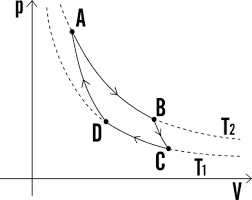
\includegraphics[width=0.3\linewidth]{immagini/screenshot002}
		\label{fig:screenshot002}
	\end{figure}
	\begin{itemize}
		\item $AB$ assorbe calore $Q_2$ dalla sorgente a temperatura maggiore $T_2$
		\item $BC$ espande adiabaticamente 
		\item $CD$ cede calore $Q_1$ alla sorgente a temperatura inferiore $T_1$
		\item $DA$ comprime adiabaticamente riportando il fluido alle condizioni iniziali
	\end{itemize}
	Thompson e Kelvin proposero così (1848) una scala termometrica in cui la temperatura fosse indice dell'efficienza di una macchina termica ideale dove allo zero assoluto corrispondeva di fatto la temperatura dell'isoterma lungo la quale il sistema non può cedere alcuna quantità di calore.
	
	Il rendimento di una macchina termica reversibile dipende solo dalle quantità di calore scambiate durante il ciclo.
	
	Dalla definizione
	\[\eta = \dfrac{L}{Q_2} = 1 - \dfrac{Q_1}{Q_2}\]
	Per un ciclo di Carnot si osserva che 
	\[\dfrac{Q_1}{Q_2} = \dfrac{T_1}{T_2}\] 
	Ovvero ll rapporto tra le quantità di calore non è una costante universale, ma dipende dalle temperature delle due isoterme, e quindi
	\[\eta = 1 - \dfrac{T_1}{T_2}\]
	Una volta dimostrato e concordato ciò, al fine di individuare una scala termodinamica assoluta, si procede a partire da una scala termometrica arbitraria, ne sia $"t"$ l'indice. 
	
	Si consideri a questo punto un ciclo di Carnot operante tra $t_1$ e $t_2$ con $t_1>t_2$, in virtù di quanto esposto poco sopra si può scrivere i calori scambiati sono funzione delle temperature estremali del ciclo
	\[\left|\dfrac{Q_1}{Q_2}\right| = f(t_1,t_2)\]
	Si identifichi ora uno nuovo ciclo di Carnot operante tra $t_1$ e $t_3(<t_2)$, varrà sempre
	\[\left|\dfrac{Q_1}{Q_3}\right| = f(t_1,t_3)\]	
	Identificando una nuova macchina termica che lavori tra $t_2$ e $t_3$ si può ancora una volta scrivere
	\[\left|\dfrac{Q_2}{Q_3}\right| = f(t_2,t_3)\]	
	Ne segue che
	\[\left|\dfrac{Q_1}{Q_2}\right| = \left|\dfrac{Q_1}{Q_3}\right|\cdot\left|\dfrac{Q_3}{Q_2}\right| = \dfrac{f(t_1,t_3)}{f(t_2,t_3)}\]	
	Per cui
	\[f(t_1,t_2) = \dfrac{f(t_1,t_3)}{f(t_2,t_3)}\]
	Affinché sia verificata l'uguaglianza, se il membro di sinistra non dipende da $t_3$, allora anche il membro di destra non deve dipenderne: dato che questa quantità è stata scelta ad arbitrio si assumerà costante. \newline
	
	A questo punto si definisce una funzione $\theta$ tale che
	\[\theta(t) = kf(t,t_3)\]
	In modo che 
	\[\left|\dfrac{Q_1}{Q_2}\right| = \dfrac{\theta(t_1)}{\theta(t_2)}\]
	Poiché si è imposta essere la scala in $"t"$ totalmente arbitraria, si può introdurre grazie a questa una nuova scala di temperature, in modo che 
	\[\left|\dfrac{Q_1}{Q_2}\right| = \dfrac{\theta_1}{\theta_2}\]
	Dal momento che la nuova scala si basa sulle proprietà termodinamiche del ciclo di Carnot, viene chiamata \textbf{scala termodinamica}.  
	
	Poiché per un ciclo di Carnot vale 
	\[\dfrac{Q_1}{Q_2} = \dfrac{T_1}{T_2}\] 
	Allora si avrà necessariamente 
	\[\dfrac{\theta_1}{\theta_2} = \dfrac{T_1}{T_2}\]
	Si ottiene la scala assoluta se si impone che alla temperatura del punto triplo dell'acqua l'indice di tale scala segni 273.16 a \SI{0.6117}{\kilo\Pa}. 
	
	In ogni caso si devono fissare dei valori di temperatura di riferimento riproducibili secondo le normative IPTS68 e ITS90, quest'ultima in particolare si estende fino a \SI{0.65}{\kelvin} ed è garanzia di maggiore precisione.
\end{adjustwidth}
\newpage
\section{Termometri a liquido}
\begin{adjustwidth}{2in}{}
	I termometri a liquido sono sensori di temperatura costituiti da un bulbo di vetro a parete sottile che racchiude un liquido termometrico. 
	\[\underset{T}{\rightarrow}\boxed{}\underset{x}{\rightarrow}\]
	Il loro funzionamento si basa sulla legge della dilatazione termica dei fluidi.
	\begin{figure}[H]
		\centering
		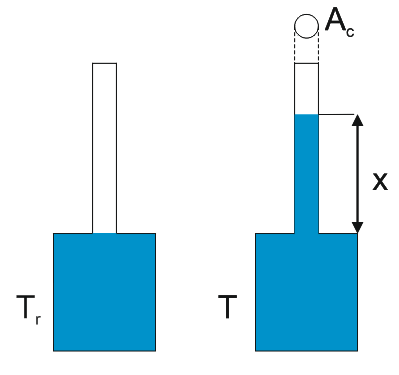
\includegraphics[width=0.2\linewidth]{immagini/screenshot003}
		\label{fig:screenshot003}
	\end{figure}
	\[\dfrac{\Delta V}{V_r} = \alpha_d(T-T_r) \qquad \Delta V = A_cx\]
	In cui
	\begin{itemize}
		\item $\Delta V$ è la variazione di volume 
		\item $V_r$ è il volume alla temperatura di riferimento
		\item $\alpha_d$ è il coefficiente di dilatazione volumica
		\item $A_c$ è l'area del capillare
		\item $x$ è l'altezza della colonna liquida 
	\end{itemize}
	Per risalire all'uscita
	\[\Delta V = A_cx = V_r\alpha_d(T-T_r)\]
	\[x = \dfrac{V_r\alpha_d(T-T_r)}{A_c}\]
	La sensibilità è sempre la derivata dell'uscita rispetto all'ingresso, per cui
	\[S = \dfrac{dx}{dT} = \dfrac{V_r\alpha_d}{A_c}\]
	Per aumentare la sensibilità sarà necessario diminuire la sezione del capillare o	costruire un bulbo di maggiore volume, tuttavia questo intaccherà inevitabilmente le caratteristiche metrologiche dinamiche, si era definito
	\[\tau = \dfrac{m \cdot c}{kA_{sc}}\]
	In cui
	\begin{itemize}
		\item $m$ è la massa del fluido
		\item $c$ è il calore specifico
		\item $k$ è il coefficiente di scambio termico
		\item $A_{sc}$ è la superficie di scambio termico
	\end{itemize}
	Per diversi range di temperatura si utilizzano
	\begin{itemize}
		\item Galistano (ex Mercurio) da \SIrange{-40}{540}{\celsius}
		\item Alcol fino a \SI{-60}{\celsius}
		\item Toluolo fino a \SI{-90}{\celsius}
		\item Miscele di propano e propilene \SI{-190}{\celsius}
	\end{itemize}
\end{adjustwidth}
\newpage
\section{Termometri bimetallici}
\begin{adjustwidth}{2in}{}
	\[\underset{T}{\rightarrow}\boxed{}\underset{\theta}{\rightarrow}\]
	Questa tipologia di termometri è costituita da due lamine di materiali differenti che vengono saldate insieme alla temperatura $T_1$, poiché i due materiali avranno diversi valori del coefficiente di dilatazione termica, si espanderanno e ritrarranno in funzione della temperatura.
	\begin{figure}[H]
		\centering
		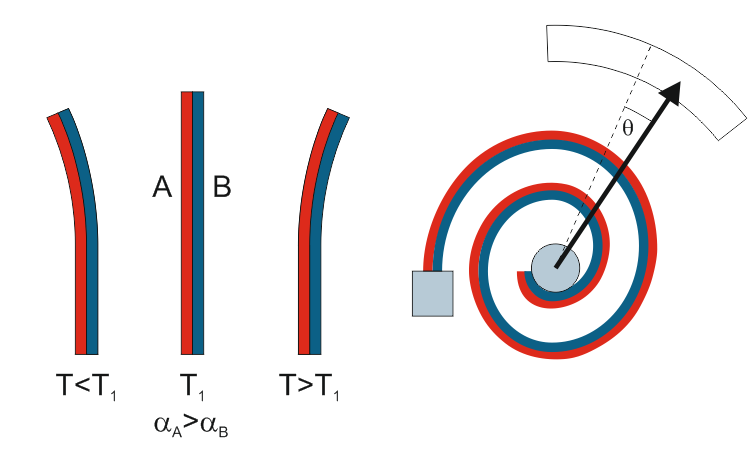
\includegraphics[width=0.5\linewidth]{immagini/screenshot004}
		\label{fig:screenshot004}
	\end{figure}
	Lamine A e B con coefficienti di dilatazione $\alpha_A$ e $\alpha_B$ determinano l'inflessione dell’insieme delle due lamine, la curvatura che assume l'elemento sensibile dipende anche dai moduli elastici dagli spessori delle lamine.\newline 
	
	Questo strumento è concettualmente simile ad un manometro Bourdon, come aumenta la lunghezze dell'elemento sensibile ne aumenterà la sensibilità. \newline 
	
	Viene utilizzato principalmente per piccoli campi di misura, essendo infatti una strumento fortemente non lineare, più piccolo è il campo di misura e più approssimabile ad una retta sarà il suo comportamento.
\end{adjustwidth}
\newpage
\section{Termometri a variazione di resistenza}
\begin{adjustwidth}{2in}{}
		\[\underset{\Delta T}{\rightarrow} \boxed{} \underset{\Delta R}{\rightarrow}\]
\end{adjustwidth}
\subsection{Termometri a metallo puro}
\begin{adjustwidth}{2in}{} 
	I termometri a metallo puro si basano sul fatto che la resistività $\rho$ varia con la temperatura $T$. 
	
	Di base il termometro a metallo puro si basa su successivi miglioramenti
	\begin{itemize}
		\item 1821: osservazione che \(\rho = f(T)\)
		\item 1871: platino come trasduttore di temperatura
		\item 1932: filo di platino avvolto intorno ad una struttura di mica isolata all'interno di un tubo di vetro
	\end{itemize}
	\begin{figure}[H]
		\centering
		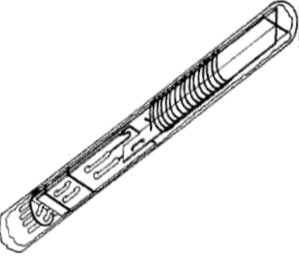
\includegraphics[width=0.3\linewidth]{immagini/Inkedscreenshot005}
		\label{fig:screenshot005}
	\end{figure}	
	Tuttavia, il principale difetto di questo strumento era l'elevato valore della costante di tempo $\tau$ dovuto alla ridotta superficie di contatto tra il punto di misura ed il metallo.
	
	\paragraph{Curva di graduazione} \mbox{} \\
	La resistività dipende dalla temperatura tramite un'equazione non lineare e per campi di misura limitati
	\[\rho_T = \rho_0(1+\alpha_1\Delta T + \alpha_2 \Delta T^2 + \dots + \alpha_n \Delta T^n)\]
	In cui 
	\begin{itemize}
		\item $\Delta T$ è la differenza tra la temperatura $T$ e quella di riferimento $T_0$
		\item $\alpha_i$ sono i coefficienti di temperatura
		\item $\rho_0$ è la resistività del sensore alla temperatura di riferimento $T_0$
	\end{itemize}
	Il numero di termini al secondo membro dipende da
	\begin{itemize}
		\item Materiale usato
		\item Campo di misura scelto
		\item Precisione ed accuratezza 
	\end{itemize}
	Per \textbf{metalli puri} l'equazione si linearizza e diviene 
	\[\rho_T = \rho_0(1+\alpha\Delta T) \Rightarrow R_T = R_0(1+\alpha\Delta T)\]
\newpage
	In questo modo la sensibilità si può scrivere come (sempre attraverso la derivata dell'uscita rispetto all'ingresso)
	\[\dfrac{dR_T}{dT} = R_0\alpha = \dfrac{\rho_0l}{A}\alpha\]
	Attraverso l'utilizzo di un metallo puro si ottiene una sensibilità costante e dipendente da un valore $\alpha\ne0$.
	
	Per aumentare la sensibilità si può
	\begin{itemize}
		\item Cambiare materiale: \(\uparrow\rho\quad\uparrow\alpha\)
		\item Modificare le dimensioni del filamento di metallo \(\uparrow l\quad\downarrow A\)
	\end{itemize}
	La curva di graduazione tuttavia varia fortemente in funzione del campo di misura:
	
	\textbf{tra \SIrange{0}{850}{\celsius}}
	\[\rho_T = \rho_0(1+\alpha_1\Delta T + \alpha_2 \Delta T^2)\]
	
	\textbf{tra \SIrange{-200}{0}{\celsius}}
	\[\rho_T = \rho_0(1+\alpha_1\Delta T + \alpha_2 \Delta T^2 + \alpha_3 \Delta T^3 + \alpha_4 \Delta T^4)\]
	
	Per arrivare alla misura di temperatura dalla misura di resistenza è necessario passare attraverso un'equazione empirica dalla soluzione iterativa
	\[T_C = \left[\dfrac{R_T-R_0}{\alpha_0R_0}\right] + \delta\left\{\left[\dfrac{t}{100}-1\right]\dfrac{t}{100}\right\} + \beta\left\{\left[\dfrac{t}{100}-1\right]\left(\dfrac{t}{100}\right)^3\right\}\]
	In cui
	\[\alpha = \dfrac{R_{100}-R_0}{100R_0}\qquad\delta = \dfrac{R_0(1+260\alpha)-R_{260}}{4.16R_0\alpha}\]
	In cui servono almeno 5 iterazioni con un $\Delta T$ di $\pm$\SI{0.001}{\celsius}
	
	\paragraph{Materiali} 
	\begin{itemize}
		\item \textbf{Rame}: lineare ma basso valore di resistività, e necessario molto materiale per aumentarne la sensibilità.
		\item \textbf{Nichel}: basso costo ma limitato campo di misura
		\item \textbf{Platino}: costoso, ampio campo di misura, minore sensibilità
		\begin{itemize}[label = \textcolor{green}{\cmark}]
			\item Chimicamente e metallurgicamente inerte comportando una maggiore stabilità del trasduttore;
			\item Un elevato valore della temperatura di fusione comporta un campo di misura maggiore;
			\item Può essere ottenuto con grado di purezza elevato comportando una modesta differenza delle curve di taratura rispetto a quella di graduazione;
			\item Modesta non linearità;
			\item A parità di resistenza di base, un termometro al Pt è caratterizzato da una minore massa rispetto a quella di un termometro realizzato in Ni comportando maggiori vantaggi per quanto riguarda la banda passante
		\end{itemize}
		\begin{itemize}[label = \textcolor{red}{\xmark}]
		\item Il coefficiente di dilatazione termica del Pt è diverso da quello degli isolanti elettrici: si dilatano in maniera differente;
		\item La deriva è dovuta alla presenza dell'ossigeno inserito per stabilizzare le impurezze; 
		sia del Pt che del materiale utilizzato come isolante elettrico;
		\item Alto costo
		\end{itemize}
	\end{itemize}
	\begin{figure}[H]
		\centering
		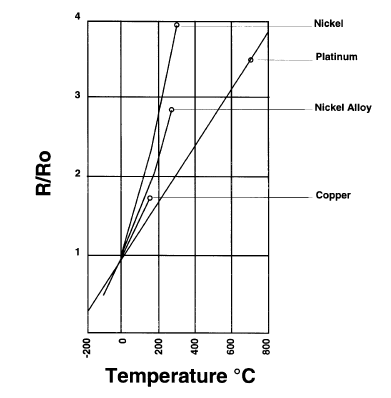
\includegraphics[width=0.3\linewidth]{immagini/screenshot006}
		\label{fig:screenshot006}
	\end{figure}
	Se la scelta del materiale ricade sul platini (e generalmente è così) lo strumento di indica con $Pt$ seguito dalla resistenza del materiale a \SI{0}{\celsius} espressa in \unit{\ohm}: \(Pt50, pT100\)
	
	\paragraph{Classificazione} \mbox{} \\
	\begin{itemize}
		\item \textbf{Standard Platinum Resistance Thermometer (SPRT)}
		\[\text{incertezza} = \pm\SI{0.001}{\celsius}\qquad\text{purezza} = 99.999\%\]
		\begin{figure}[H]
			\centering
			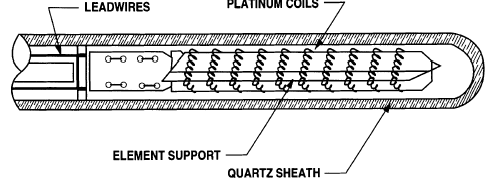
\includegraphics[width=0.5\linewidth]{immagini/screenshot007}
			\label{fig:screenshot007}
		\end{figure}
		\item \textbf{Secondary Standard Platinum Resistance Thermometer (SSPRT)}
		\[\text{incertezza} = \pm\SI{0.03}{\celsius}\]
		\begin{figure}[H]
			\centering
			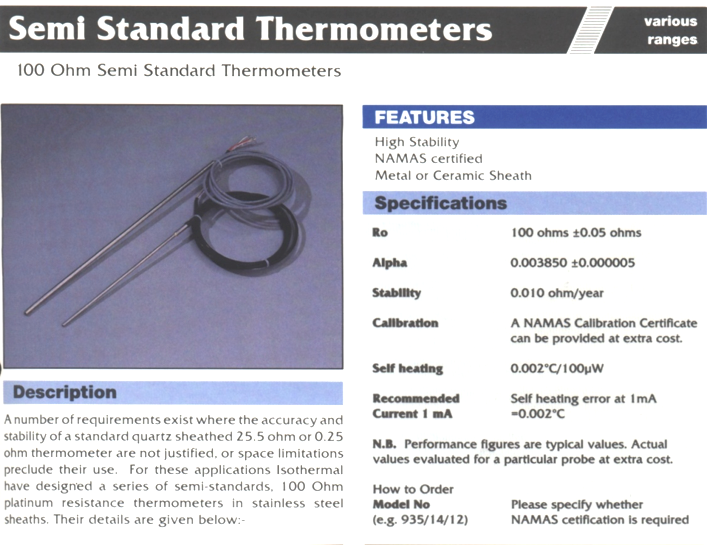
\includegraphics[width=0.5\linewidth]{immagini/screenshot008}
			\label{fig:screenshot008}
		\end{figure}
		\item \textbf{Industrial Platinum Resistance Thermometer (IPRT)}
		\[\text{incertezza} = \pm\SI{0.1}{\celsius}\]
		\begin{figure}[H]
			\centering
			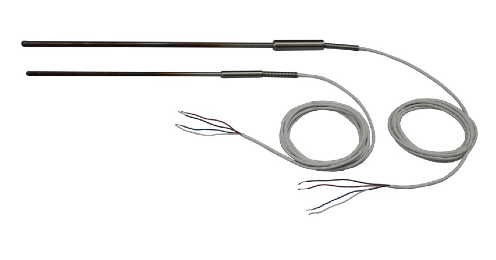
\includegraphics[width=0.3\linewidth]{immagini/screenshot009}
			\caption{Sensore a filo}
			\label{fig:screenshot009}
		\end{figure}
		\begin{figure}[H]
			\centering
			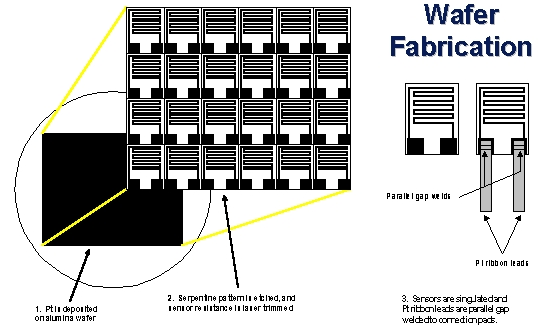
\includegraphics[width=0.3\linewidth]{immagini/screenshot010}
			\caption{Sensore a film}
			\label{fig:screenshot010}
		\end{figure}
		Il fine di quest'ultimo strumento è quello di minimizzare l'effetto delle deformazioni (grandezza di influenza) sul sensore		
	\end{itemize}
	Un'altra classificazione viene effettuata in funzione della tolleranza dei materiali
	\begin{figure}[H]
		\centering
		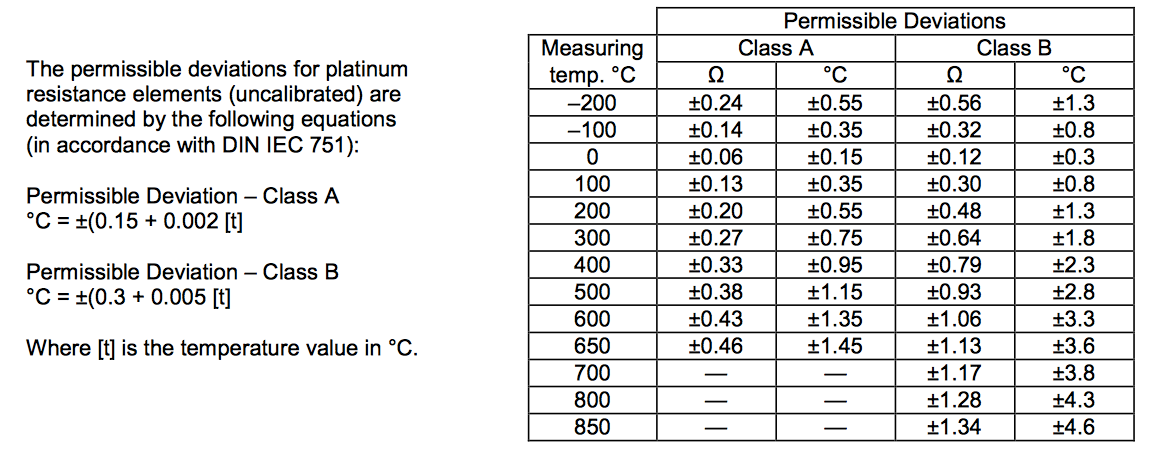
\includegraphics[width=0.5\linewidth]{immagini/screenshot011}
		\label{fig:screenshot011}
	\end{figure}
	\begin{figure}[H]
		\centering
		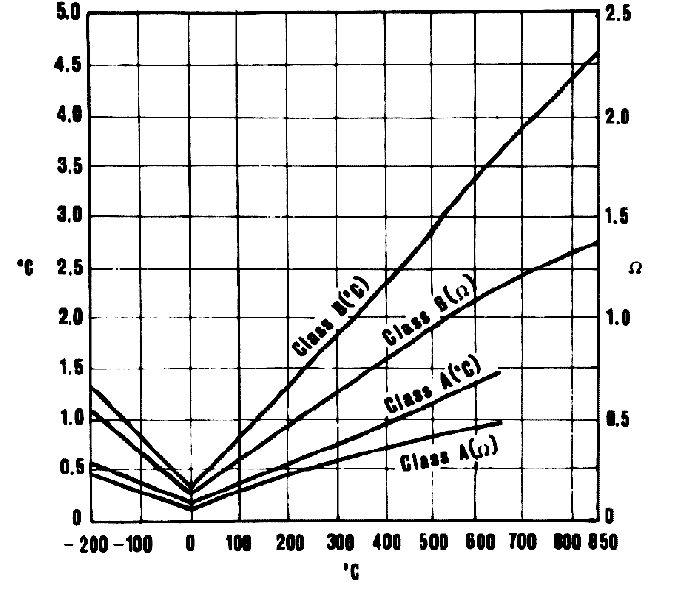
\includegraphics[width=0.5\linewidth]{immagini/screenshot012}
		\label{fig:screenshot012}
	\end{figure}
\end{adjustwidth}
\newpage
\subsection{Termistori}
\begin{adjustwidth}{2in}{} 	
	I termistori si basano su sulla variazione della conduzione elettrica in dipendenza della concentrazione di ossigeno nel materiale. \newline 
	
	Per la realizzazione dei termistori vengono utilizzati materiali quali ossidi a semiconduttore di nichel, cobalto, manganese o semiconduttori silicio o germanio drogati. \newline 
	
	In funzione della quantità di ossigeno i termistori si dividono in 
	\begin{itemize}
		\item \textbf{Di tipo P} quando un \underline{eccesso} di ossigeno causa un difetto di atomi ionizzanti (difetto Scottky).
		\item \textbf{Di tipo N} quando nel reticolo un \underline{difetto} di ossigeno determina la presenza di un eccesso di atomi ionizzati (difetto di Frankel).
	\end{itemize}
	\begin{figure}[H]
		\centering
		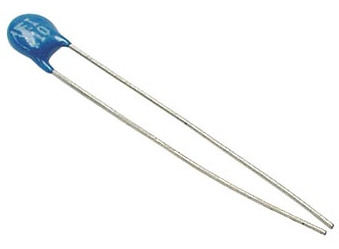
\includegraphics[width=0.2\linewidth]{immagini/screenshot013}
		\label{fig:screenshot013}
	\end{figure}
	Per la loro realizzazione si utilizzano ossidi metallici in polvere ai quali viene aggiunto un legante in modo da ottenere un impasto semiliquido che verrà poi sinterizzato. 
	
	Nella fase di sinterizzazione avviene il contatto elettrico tra i fili di connessione. 
	
	Alla fine del processo viene applicato uno strato di vetro capace di eliminare la possibilità di adsorbimento del vapore da parte degli ossidi metallici. 
	\begin{figure}[H]
		\centering
		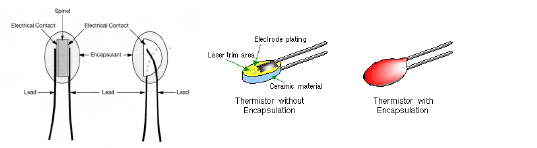
\includegraphics[width=0.5\linewidth]{immagini/screenshot014}
		\label{fig:screenshot014}
	\end{figure}
	\paragraph{Curva di graduazione} 
	\[R_T = R_0e^{\beta\left(\dfrac{T_0-T}{T_0T}\right)}\]
	Dove 
	\begin{itemize}
		\item \(\beta = [\unit{\kelvin}]\) è una costante che varia in funzione del termistore e viene definita in funzione del campo di misura.
		\item $R_0$ è la resistenza alla temperatura di rifermento $T_0(\SI{25}{\celsius})$
		\item TUTTE le temperature sono espresse in Kelvin
	\end{itemize}
	La sensibilità è
	\[S = \dfrac{dR}{dT} = -\dfrac{\beta}{T^2}R_0e^{\beta\left(\dfrac{T_0-T}{T_0T}\right)}= - \dfrac{\beta}{T^2}R_T\]
	Si nota immediatamente come la sensibilità dello strumento sia fortemente non lineare e come all'aumentare della temperatura questa diminuisca e viceversa.
	
	\paragraph{Classificazione} \mbox{} \\
	\begin{itemize}
		\item \textbf{Termistore PTC}: fusibile termico. 
		\begin{figure}[H]
			\centering
			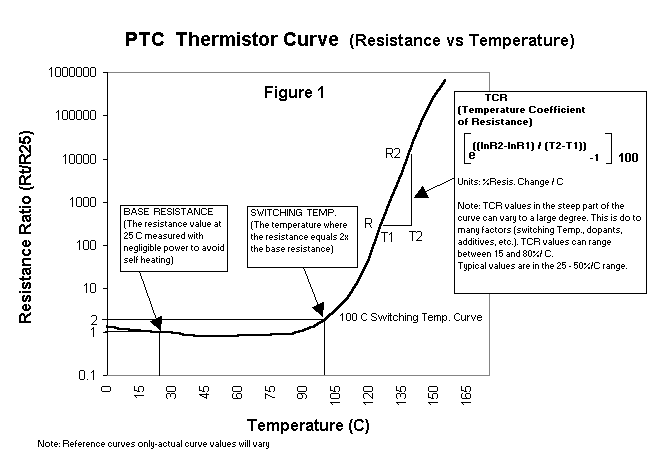
\includegraphics[width=0.3\linewidth]{immagini/screenshot015}
			\label{fig:screenshot015}
		\end{figure}
		È principalmente caratterizzato da 3 zone 
		\begin{enumerate}
			\item a sensibilità modesta -\SI{1}{\percent\per\celsius}
			\item di transizione da \SIrange{60}{120}{\celsius}
			\item a ad altissima sensibilità \SI{100}{\percent\per\celsius}
		\end{enumerate}
		\begin{figure}[H]
			\centering
			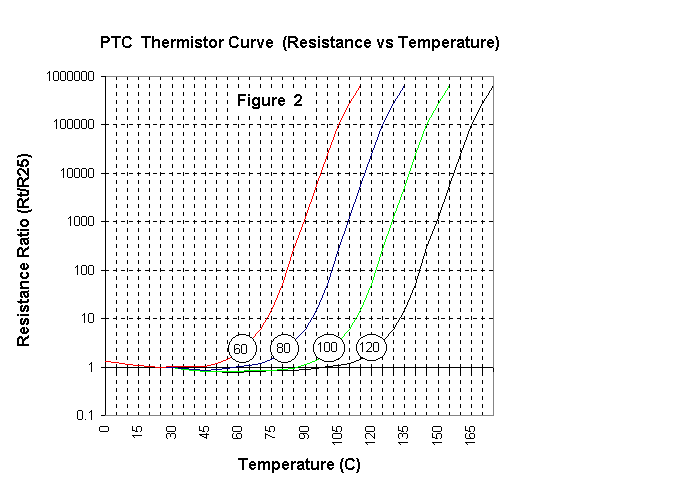
\includegraphics[width=0.3\linewidth]{immagini/screenshot016}
			\label{fig:screenshot016}
		\end{figure}
		Nella zona $3.$ la curva è quasi verticale, questo significa che ad un piccolo $\Delta T$ corrisponde un $\Delta R$ elevato: a \SI{15}{\celsius} si possono arrivare a resistenze di \SIlist{900;10}{\kilo\ohm}, la resistenza assume così valori talmente elevati da impedire alla corrente di scorrere senza che il fusibile sia danneggiato, è un fusibile riutilizzabile.
		\item \textbf{Termistore NTC}: trasduttore di temperatura. 
		
		In questo tipo di termistori dalla sensibilità elevata la curva di graduazione dipende dai materiali utilizzati e dalla durata e temperatura del processo di sinterizzazione.
		\begin{figure}[H]
			\centering
			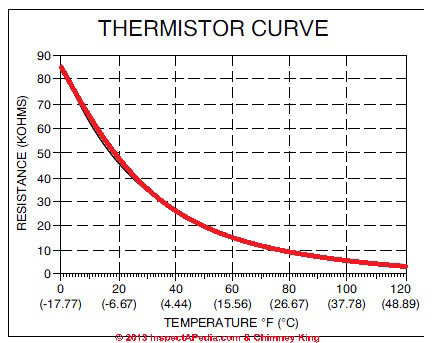
\includegraphics[width=0.3\linewidth]{immagini/screenshot017}
			\label{fig:screenshot017}
		\end{figure}
		Il campo di misura è compreso tra \SIlist{-100;+300}{\celsius}		
	\end{itemize}
\end{adjustwidth}
\newpage
\subsection{Termistori vs Pt100}
\begin{adjustwidth}{2in}{} 	
	\begin{itemize}
		\item Il valore della resistenza a temperatura ambiente di un termistore (\SI{10}{\kilo\ohm}) è maggiore di
		quello di un termometro a filo metallico (\SI{100}{\ohm}) 
		\item La sensibilità di un termistore (\SI{3}{\percent\per\celsius}) è maggiore
		di quella di un termometro a filo metallico (\SI{0.4}{\percent\per\celsius})
		\item La curva di graduazione di un termistore non può essere assunta lineare al
		contrario di quella dei termometri a filo metallico
		\item La misura della resistenza a 2 fili può essere utilizzata con il termistore (ottenendo una misura più precisa) mentre è da evitare nel caso di termometri al platino (Pt50, Pt100)
	\end{itemize}	
	\begin{center}
		Termistore 3 - 1 Metallo puro
	\end{center} 
	\begin{figure}[H]
		\centering
		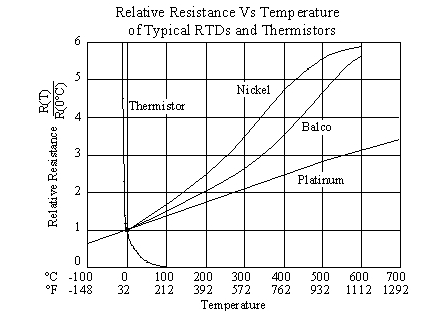
\includegraphics[width=0.7\linewidth]{immagini/screenshot018}
		\caption{Curve di graduazione dei principali termometri metallici}
		\label{fig:screenshot018}
	\end{figure}
\end{adjustwidth}
\newpage
\section{Termocoppie}
\begin{adjustwidth}{2in}{} 	
	La termocoppia si basa sull'effetto Seeback. 
	\[\underset{\Delta T}{\rightarrow} \boxed{} \underset{\Delta V}{\rightarrow}\]
	
	L'effetto Seeback si basa sulla diffusione di elettroni attraverso l'interfaccia di due metalli saldati assieme attivata da una differenza di temperatura. 
	
	Il materiale che riceve elettroni (accettore) diventa all'interfaccia negativo, mentre il materiale che fornisce elettroni (donatore) diviene all'interfaccia positivo. 
	\begin{figure}[H]
		\centering
		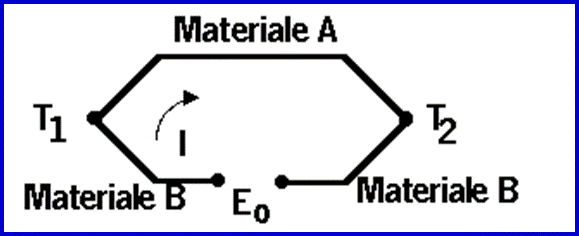
\includegraphics[width=0.2\linewidth]{immagini/screenshot019}
		\label{fig:screenshot019}
	\end{figure}	
	L'intensità di diffusione degli elettroni dipende dalla temperatura della giunzione in questo modo il potenziale elettrico sviluppato fornisce un'indicazione sulla temperatura mentre il campo elettrico impedisce l'ulteriore migrazione degli elettroni quando viene raggiunto un valore sufficientemente alto della differenza di potenziale. \newline 
	
	La \textbf{curva di graduazione} delle termocoppie è descritta da 
	\[\Delta V = C_1(T_1-T_2) + C_2(T_1^2-T_2^2)\]
	E non è lineare.
\end{adjustwidth}
%\newpage
\subsection{Leggi delle termocoppie}
\paragraph{I Legge}
\begin{definizione} 
	Un circuito di una termocoppia deve prevedere almeno due materiali e due giunzioni.
\end{definizione}

	\begin{figure}[H]
		\centering
		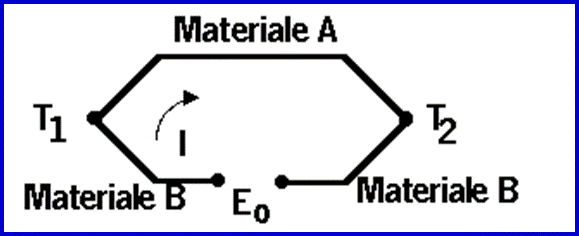
\includegraphics[width=0.5\linewidth]{immagini/screenshot020}
		\label{fig:screenshot020}
	\end{figure}
	\[E_0 = e_{B/A}T_1 + e_{A/B}T_2 \qquad  e_{B/A} = - e_{A/B} = f(T) \Rightarrow E_0 = e_{B/A}(T_1 - T_2)\]
	Con $e_{x/y}$ coefficiente termico che va dal materiale $x$ al materiale $y$.
\newpage
\paragraph{II Legge} 		
\begin{definizione}		
	La tensione $E_0$ fornita da una termocoppia dipende solo dalla differenza delle
	temperature delle giunzioni $(T_1-T_2)$, mentre è del tutto indipendente da
	qualsiasi altra temperatura presente nel circuito.
\end{definizione}	

	\begin{figure}[H]
		\centering
		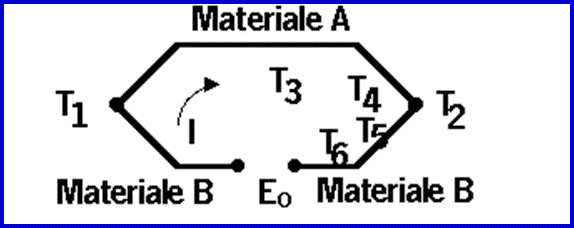
\includegraphics[width=0.5\linewidth]{immagini/screenshot021}
		\label{fig:screenshot021}
	\end{figure}
	
\paragraph{III Legge} 		
\begin{definizione}		
	Se un terzo materiale C viene introdotto in un ramo del circuito di materiale A
	e le due nuove giunzioni A/C e C/A sono mantenute alla stessa temperatura,
	la $E_0$ non subisce variazioni.
\end{definizione}		
	\[E_0 = e_{B/A}T_1 + e_{A/C}T_i + e_{C/A}T_j + e_{A/B}T_2\]
	\[e_{B/A} = - e_{A/B} \qquad e_{A/C} = - e_{C/A}\]
	\[E_0 =  e_{B/A}(T_1-T_2) + e_{A/C}(T_i-T_j)\]
	\begin{figure}[H]
		\centering
		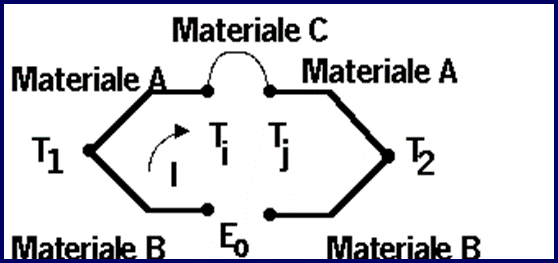
\includegraphics[width=0.5\linewidth]{immagini/screenshot022}
		\label{fig:screenshot022}
	\end{figure}
	La III legge diviene utile non appena la zona tra $T_2$ e $T_1$ è ampia, in questo modo il metallo puro viene utilizzato soltanto per la realizzazione dei giunti mentre il collegamento tra questi viene realizzato tramite lo stesso materiale, meno nobile e meno costoso.  
\newpage	
\paragraph{IV Legge} 		
\begin{definizione}		
	Se un terzo materiale C viene introdotto in una giunzione A/B e le due nuove
	giunzioni A/C e C/B sono mantenute alla stessa temperatura $T_1$, la $E_0$ non
	subisce variazioni.
\end{definizione}
	\[E_0 = e_{B/C}T_1 + e_{C/A}T_1+e_{A/B}T_2\]
	\[e_{C/A} = e_{C/B} + e_{B/A}\]
	\[E_0 = e_{B/A}(T_1-T_2) \]
	\begin{figure}[H]
		\centering
		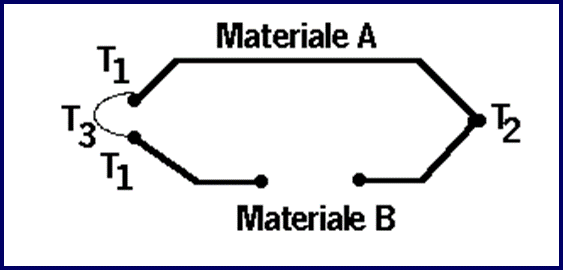
\includegraphics[width=0.5\linewidth]{immagini/screenshot023}
		\label{fig:screenshot023}
	\end{figure}
	Questa legge permette di saldare fisicamente il giunto: utilizzando un terzo materiale (il metallo fusibile), l'output dello strumento non varia perché i tre materiali si trovano tutti alla stessa temperatura. 
	
\paragraph{V Legge} 		
\begin{definizione}		
	Se una termocoppia con i giunti alle temperature $T_1$ e $T_2$ genera una tensione
	$(E_0)_{1-2}=f(T_1-T_2)$ ed un'altra termocoppia, dello stesso tipo, sottoposta a
	temperature $T_2$ e $T_3$ genera una tensione $(E_0)_{2-3}=f(T_2-T_3)$, la tensione $(E_0)_{1-3}$ è data da:
	\[(E_0)_{1-3} = f(T_1-T_3) = (E_0)_{1-2} + (E_0)_{2-3} \]
\end{definizione}	
	\begin{figure}[H]
		\centering
		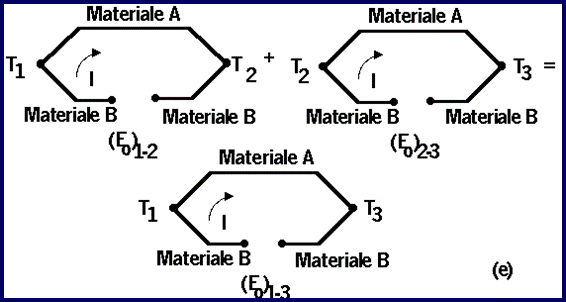
\includegraphics[width=0.5\linewidth]{immagini/screenshot024}
		\label{fig:screenshot024}
	\end{figure}		
	\[\boxed{\begin{matrix}
		\Delta T_{1,2} &        &\Delta T_{2,3}    &      \\
		(E_0)_{1,2} & + & (E_0)_{2,3} & = (E_0)_{1,3}
	\end{matrix}}\]
	Come se fosse un'unica termocoppia. \newline 
	
	Per quale motivo è importante questa legge?
	Questa legge permette di individuare una temperatura incognita a partire da una termocoppia non riferita attraverso l'utilizzo di una termocoppia virtuale che sia riferita tra le stesse temperatura.
\newpage	
	L'uscita della termocoppia è dipendente dall'ingresso mediante questa formula
	\[E_0 = e_{x/y}\Delta T\]
	Dove il termine $e_{x/y}$ non è costante.
	
	La misura del $\Delta T$ si esegue quindi attraverso la misura di un $E_0$ che avviene attraverso un termine incognito. \newline
	
	Sia ad esempio una termocoppia operante tra $T_1$ e $T_2$ che misura una tensione di \SI{0.15}{\volt}. Si vuole conoscere $T_1$ sapendo che $T_2\ne T_{rif}$ non è la usuale temperatura di riferimento. 
	
	Si utilizza allora una termocoppia "virtuale" operante tra $T_2$ e $T_3=T_{rif}$, in cui quest'ultima è l'usuale temperatura di riferimento. 
	Attraverso le\textit{tabelle delle termocoppie} si risale così alla tensione misurata da questa termocoppia tra queste temperature, magari \SI{0.25}{\volt}, in questo modo, grazie alla V legge: 
	\[0.15_{reale} + 0.25_{virtuale} = \SI{0.4}{\volt}\]
	Con questo valore di tensione si può così rientrare in tabella ed individuare il $T_1$ incognito. 
	 
\paragraph{VI Legge} 		
\begin{definizione}		
	Se una termocoppia che utilizza materiali A/C viene sottoposta alla differenza
	di temperatura $(T_1 - T_2)$ e genera una $(E_0)_{A/C}$ ed un'altra termocoppia C/B,
	sottoposta alla stessa differenza di temperature genera una $(E_0)_{C/B}$, allora una
	termocoppia A/B, sottoposta alla stessa differenza di temperature genera una $(E_0)_{A/B}$ uguale a:
	\[(E_0)_{A/B} = (E_0)_{A/C} + (E_0)_{C/B}\]
\end{definizione}		
	\begin{figure}[H]
		\centering
		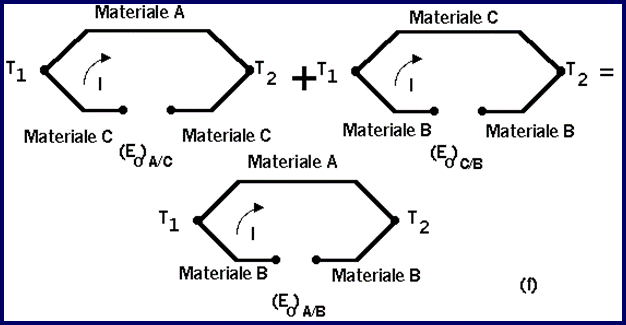
\includegraphics[width=0.5\linewidth]{immagini/screenshot025}
		\label{fig:screenshot025}
	\end{figure}

\newpage
\subsection{Classificazione}
\begin{adjustwidth}{2in}{}
% \nointerlineskip\leavevmode
	Esistono3 principali classi di termocoppie, in base al metallo con cui vengono realizzate
	\begin{itemize}
		\item Metalli di base (Cu, Fe, Mn) con portata massima fino a \SI{1000}{\celsius}
		\item Metalli nobili (Pt, Ir) con portata massima fino a \SI{2000}{\celsius}
		\item Metalli refrattari (W, Ta,Mo) con portata massima fino a \SI{2800}{\celsius}
	\end{itemize}
	Tra queste le più largamente usate sono le termocoppie di \textbf{tipo K} e di \textbf{tipo J}. \newline 
	
	\begin{itemize}
		\item \textbf{Tipo K}
		\[\SIrange{-200}{1260}{\celsius} \qquad S = \SI{41.0}{\micro\volt\per\celsius}\]
		\begin{itemize}
			\item \textbf{Chromel NiCr}: \textcolor{yellow}{positivo}
			\item \textbf{Alumel NiAl}: \textcolor{red}{negativo}
		\end{itemize}
		
		\item \textbf{Tipo J}
		\[\SIrange{-40}{750}{\celsius} \qquad S = \SI{51.7}{\micro\volt\per\celsius}\]
		\begin{itemize}
			\item \textbf{Ferro}: \textcolor{gray}{positivo} (bianco)
			\item \textbf{Costantana CuNi}: \textcolor{red}{negativo}
		\end{itemize}
	\end{itemize}
	
	Per quanto riguarda l'impiego, si sceglie la tipologia di termocoppia in funzione dell'ambiente di destinazione: 
	\begin{itemize}
		\item \underline{Ambienti riducenti}: termocoppie J
		\item \underline{Ambienti ossidanti}: termocoppie K (ed E)
		\item Tra \SIlist{-40;400}{\celsius} indipendentemente dall'ambiente: termocoppie T
	\end{itemize}
	\begin{figure}[H]
		\centering
		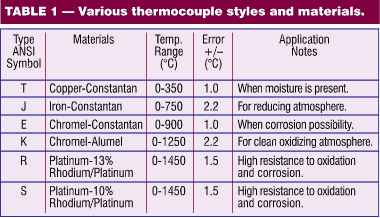
\includegraphics[width=0.5\linewidth]{immagini/screenshot026}
		\label{fig:screenshot026}
	\end{figure}	
\end{adjustwidth}
\newpage
\subsection{Giunto di riferimento}
\begin{adjustwidth}{2in}{}	
	Affinché la termocoppia sia efficace si deve realizzare un giunto di riferimento. 
	
	Questo consta nella realizzazione e nel mantenimento del "giunto freddo" ad una temperatura nota attraverso diverse applicazioni tecniche. 
	
	\paragraph{Vaso Dewar} \mbox{} \\
	Vaso adiabatico contenente una miscela di acqua e ghiaccio, per mantenere l'equilibrio termico (\SI{0}{\celsius}) è necessario che l'operatore aggiunga ghiaccio ed rimuova l'acqua in eccesso. 
	
	L'incertezza associata a questo strumento è di \SI{0.1}{\celsius}
	\begin{figure}[H]
		\centering
		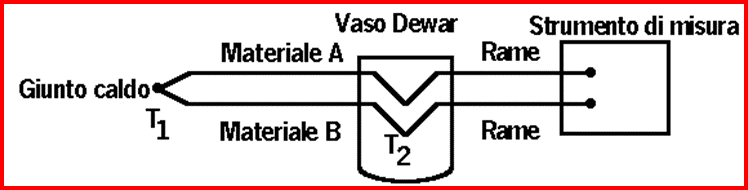
\includegraphics[width=0.5\linewidth]{immagini/screenshot027}
		\label{fig:screenshot027}
	\end{figure}
	
	\paragraph{Cella Peltier} \mbox{} \\
	Il giunto freddo viene posto all'interno di un contenitore nel quale è presente acqua satura d'aria mantenuta a \SI{0}{\celsius} per effetto Peltier: 
	\begin{definizione}
		Fenomeno termoelettrico per cui una corrente elettrica che scorre tra due metalli o semiconduttori differenti posti in contatto (giunzione Peltier) produce un trasferimento di calore. È l'opposto dell'Effetto Seebeck. 
	\end{definizione}
	Il passaggio di corrente determina un assorbimento di calore dal metallo del giunto. 
	\begin{figure}[H]
		\centering
		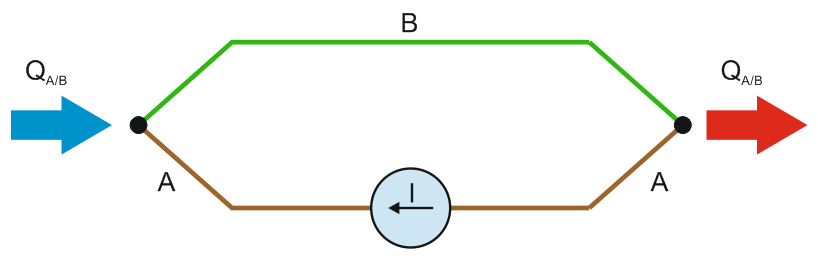
\includegraphics[width=0.5\linewidth]{immagini/screenshot028}
		\label{fig:screenshot028}
	\end{figure}
	 Controllando la corrente si riesce a stabilizzare la temperatura.
\newpage	 
	 \paragraph{Compensazione con circuito a ponte} \mbox{} \\
	 La tensione $E_0$ della termocoppia a $T_1$ si misura in serie all'uscita di un ponte di Wheatstone le cui resistenze vengono scelte per essere in equilibrio alla temperatura $T_2$ di riferimento. 
	 
	 Un ramo del ponte di Wheatstone è occupato da un termistore applicato ad  un blocco isotermo a $T_2$, se tale temperatura varia viene a crearsi una variazione di tensione $E_1$ - dovuta allo stesso termistore - ed una variazione $E_2$  dovuta alla variazione di temperatura del giunto freddo.
	 
	 Il sistema è così dimensionato in modo che 
	 \[E_1=-E_2\]
	 \begin{figure}[H]
	 	\centering
	 	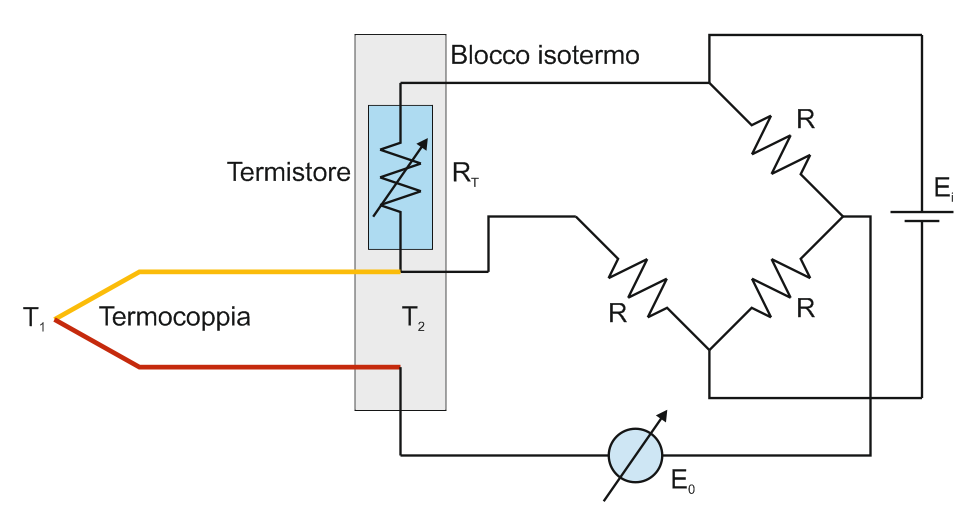
\includegraphics[width=0.5\linewidth]{immagini/screenshot029}
	 	\label{fig:screenshot029}
	 \end{figure}
	 
	 
	 \paragraph{Compensazione con circuito integrato} \mbox{} \\
	  Misura la temperatura del giunto di riferimento tramite termometro a circuito integrato e fornisce una tensione uguale in modulo ma in verso opposto alla  tensione generata dalla termocoppia a causa della variazione della temperatura del giunto di riferimento, questo posto all'interno del chip.	  
	  \begin{figure}[H]
	  	\centering
	  	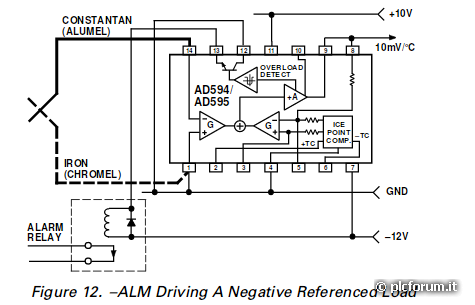
\includegraphics[width=0.5\linewidth]{immagini/screenshot030}
	  	\label{fig:screenshot030}
	  \end{figure}
\end{adjustwidth}
\newpage
\subsection{Giunto di misura}
\begin{adjustwidth}{2in}{}	  
	La scelta del diametro dei fili dipende dalla risposta dinamica desiderata e dalle caratteristiche corrosive dell'ambiente. 
	\begin{figure}[H]
		\centering
		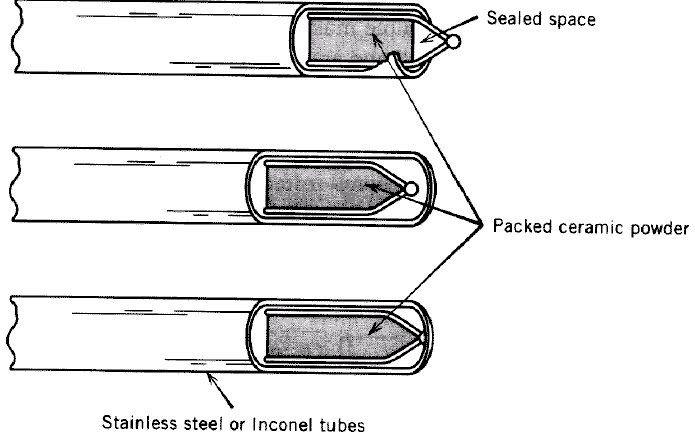
\includegraphics[width=0.5\linewidth]{immagini/screenshot031}
		\label{fig:screenshot031}
	\end{figure}
	Si potrà così avere un giunto di misura
	\begin{itemize}
		\item Non protetto
		\item Collegato a massa
		\item Isolato
	\end{itemize}
\end{adjustwidth}
%\newpage
\subsection{Cavi di Compensazione}
\begin{adjustwidth}{2in}{}		
	I cavi di compensazione devono prefiggersi due scopi: 
	\begin{enumerate}
		\item Economicità: infatti il grado di purezza dei fili può essere inferiore di quello
		dei fili costituenti la termocoppia
		\item Praticità: ottenere una maggiore facilità nella realizzazione dei collegamenti grazie alla maggiore flessibilità dei cavi di compensazione rispetto ai cavi delle
		termocoppie
	\end{enumerate}
	\begin{figure}[H]
		\centering
		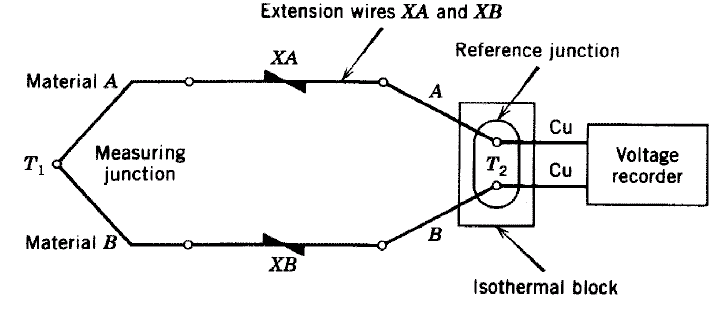
\includegraphics[width=0.3\linewidth]{immagini/screenshot032}
		\label{fig:screenshot032}
	\end{figure}
	\begin{figure}[H]
		\centering
		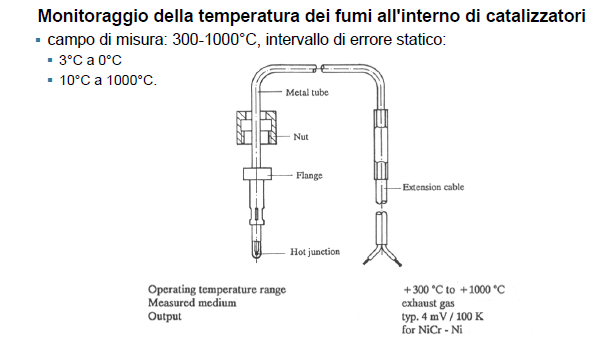
\includegraphics[width=0.7\linewidth]{immagini/screenshot033}
		\label{fig:screenshot033}
	\end{figure}
\end{adjustwidth}
\newpage
\section{Termometri a circuito integrato}
\begin{adjustwidth}{2in}{}	
	I termometri a circuito integrato fanno uso di transistor.
	\[\underset{T}{\rightarrow}\boxed{}\underset{V}{\rightarrow}\boxed{}\underset{I}{\rightarrow}\]
	Un transistor è formato da tre strati di silicio, nello strato centrale c'è un drogaggio opposto agli altri due.
	\begin{figure}[H]
		\centering
		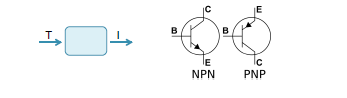
\includegraphics[width=0.5\linewidth]{immagini/screenshot034}
		\label{fig:screenshot034}
	\end{figure}	
	Ad ogni strato è associato un terminale: base (centrale), collettore ed
	emettitore (esterni). \newline 
	
	Il principio di funzionamento si fonda sulla possibilità di controllare la corrente elettrica che attraversa il transistor mediante l'applicazione di una tensione tra i suoi terminali. \newline 
	
	Il valore della tensione base-emettitore varia con la temperatura
	\[V = AT + B + Ce^{-\alpha(T-T_0)}\]
	Se varia la temperatura varia la tensione, al variare della tensione varia la corrente che attraversa il transistor: circuito integrato a conversione diretta di intensità di corrente.  
	\begin{figure}[H]
		\centering
		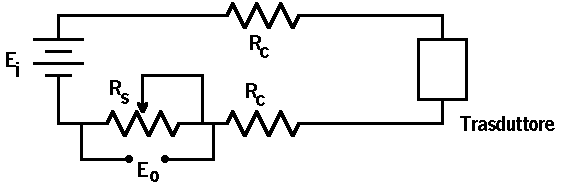
\includegraphics[width=0.3\linewidth]{immagini/screenshot035}
		\label{fig:screenshot035}
	\end{figure}
	\[E_0 = IR_s = S_iT_\alpha R_s = S_tT_\alpha\]
	Dove
	\begin{itemize}
		\item $I$ è l'intensità di corrente generata alla temperatura assoluta $T_a$,
		\item $R_s$ è la resistenza posta in serie, ai capi della quale è misurata la tensione in
		uscita,
		\item $T_a$ è la temperatura assoluta,
		\item $S_i$ è il fattore di sensibilità in corrente del trasduttore
		\item $S_t$ è il fattore di sensibilità in tensione del circuito.
	\end{itemize}
\end{adjustwidth}	
\newpage	
\begin{figure}[H]
	\centering
	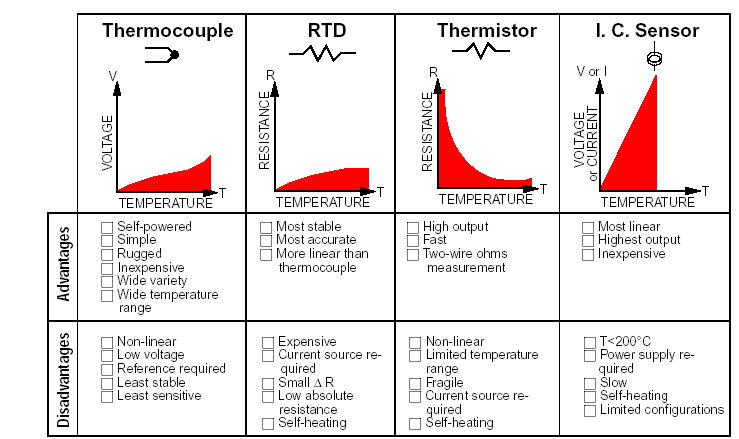
\includegraphics[width=1\linewidth]{immagini/screenshot036}
	\caption{Termometri a confronto}
	\label{fig:screenshot036}
\end{figure}


\section{Termometri chimici}
\subsection{A cristalli liquidi}
\begin{adjustwidth}{2in}{}	
	\textbf{Cristalli liquidi}: composti organici che non passano direttamente dallo stato liquido al quello stato solido ma attraversano prima stato di aggregazione intermedio tra la fase liquida e quella cristallina. \newline 
	
	I cristalli liquidi sono caratterizzati da un'organizzazione molecolare intermedia tra la quasi totale assenza di ordine (liquido) e l'elevato grado di ordine (cristalli). \newline 
	
	Si individuano due tipo di cristalli liquidi
	\begin{itemize}
		\item \textbf{Nematici}: molecole allungate distribuite secondo una direzione con un certo ordine
		
		\item \textbf{Colesterici}: strati adiacenti orientati in modo
		da formare un angolo tale che l'insieme delle direzioni individuate dalle molecole, spostandosi ortogonalmente agli strati, assume un andamento ad elica. 
		
		La distanza tra due piani consecutivi con stesso orientamento è il passo $p$ dell'elicoide.		
		\begin{figure}[H]
			\centering
			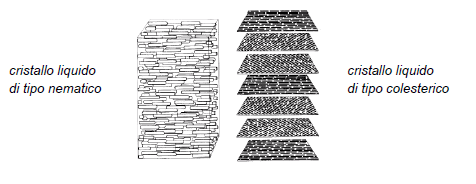
\includegraphics[width=0.5\linewidth]{immagini/screenshot037}
			\label{fig:screenshot037}
		\end{figure}
		
		\paragraph{Funzionamento} \mbox{} \\
		I cristalli liquidi mostrano una capacità di riflettere selettivamente la luce incidente
		\[p=n\lambda\]
		Al variare della temperatura varia il passo dell'elica e quindi $\lambda$: viene riflesso un colore differente. \newline
		
		Questo tipo di trasduttori si indicano con sigle tipo R35C1W dove
		\begin{itemize}
			\item 35 indica l'\textit{event temperature}: la temperatura alla quale il cristallo assume il colore rosso
			\item 1 indica la \textit{bandwidth}: la variazione in \unit{\celsius} alla quale si ha la conversione in blu
		\end{itemize}
		\begin{figure}[H]
			\centering
			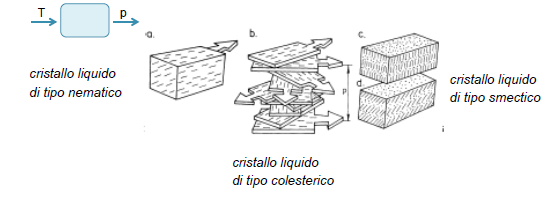
\includegraphics[width=0.5\linewidth]{immagini/screenshot038}
			\label{fig:screenshot038}
		\end{figure}
		Il rilevamento delle diverse aree di colore assunto dai cristalli liquidi, condotto con mezzi fotografici o con metodi più recenti di acquisizione di immagini da parte di sistemi automatici, insieme ai dati di taratura relativi al particolare cristallo liquido utilizzato, consente il rilievo dei campi di temperatura con intervalli di incertezza pari a \SI{0.1}{\celsius}.
		
		Per assicurare detti intervalli di incertezza lo sperimentatore deve porre particolare attenzione affinché sia assicurato un contatto certo tra pelle e pellicola a cristalli liquidi.
	\end{itemize}
\end{adjustwidth}
\subsection{A cambiamento di stato di aggregazione}
\begin{adjustwidth}{2in}{}	
	Il principio fisico alla base di questi termometri è il cambiamento di stato solido - liquido di alcune sostanze (bromo/cloro-nitrobenzene)  che avviene ad una temperatura funzione delle proporzione della miscela. 
	
	Hanno un campo di misura da \SIrange{34}{37}{\celsius} con una risoluzione di \SI{0.1}{\celsius}.
	
	Viene utilizzato principalmente come monitoraggio: ad una determinata temperatura un elemento passa allo stato solido ed espandendo rompe il vetro nel quale è contenuto.
	\begin{figure}[H]
		\centering
		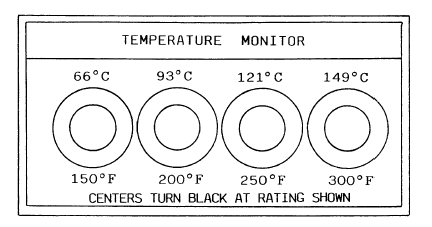
\includegraphics[width=0.5\linewidth]{immagini/screenshot039}
		\label{fig:screenshot039}
	\end{figure}
\end{adjustwidth}
\newpage
\section{Termometri a ultrasuoni}
\begin{adjustwidth}{2in}{}	
	I termometri ad ultrasuoni sono adatti ad una misura "non-a-contatto" e si basano sul mezzo come trasduttore di un'onda di segnale che varia con la temperatura. 
	
	Ad un ampio campo di misura (fino a \SI{3000}{\celsius}) corrispondono tuttavia problemi di interferenza di natura meccanica e di valutazione di una temperatura media del conduttore (2-5~\si{\centi\metre}).
	\begin{figure}[H]
		\centering
		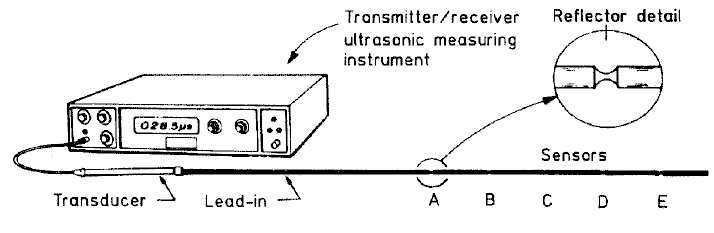
\includegraphics[width=0.5\linewidth]{immagini/screenshot040}
		\label{fig:screenshot040}
	\end{figure}
\end{adjustwidth}
%\newpage
\section{Taratura}
\begin{adjustwidth}{2in}{}
	\nointerlineskip\leavevmode
	\paragraph{Per confronto} \mbox{} \\
	Si utilizza un SPRT di alto grado in pozzetto di calibrazione
		\begin{figure}[H]
			\centering
			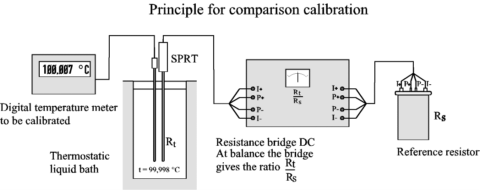
\includegraphics[width=0.5\linewidth]{immagini/screenshot041}
			\label{fig:screenshot041}
		\end{figure}
		
		\paragraph{A punto di solidificazione ed ebollizione} \mbox{} \\
		\textbf{Termocoppia Autocalibrante}\\
		\begin{enumerate}
		\item Il trasduttore immerso in metallo puro fuso
		\item Il metallo viene fatto raffreddare
		\item Quando il metallo si solidifica si ha una uscita costante nel tempo: l'uscita è nulla, non si misura niente
		\item A questo punto essendo nota la temperatura di fusione è possibile correggere.
		\end{enumerate}
		Necessario condurre più prove con materiali puri. 
		
		Per campi di temperatura minori si usa il passaggio da vapore a liquido.		
		\begin{figure}[H]
			\centering
			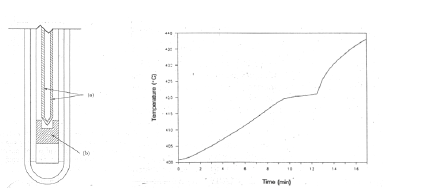
\includegraphics[width=0.5\linewidth]{immagini/screenshot042}
			\label{fig:screenshot042}
		\end{figure}
		
		\paragraph{A filo fondente} \mbox{} \\
		Metodo utilizzato nelle termocoppie: il giunto caldo viene realizzato con un terzo materiale puro di cui si conosce l'esatta temperatura di fusione. 
		
		Appena questo metallo fonde non si misura più alcuna tensione: il valore misurato nell’istante precedente alla fusione equivale alla temperatura di fusione del metallo posto nel giunto di misura, in questo modo è possibile correggere la misura.
	\end{adjustwidth}

	{\LARGE \textbf{NOTE}}
\end{document}
